\documentclass[tikz]{standalone}%

\usepackage[utf8]{inputenx}%  http://ctan.org/pkg/inputenx
% Euler for math | Palatino for rm | Helvetica for ss | Courier for tt
\renewcommand{\rmdefault}{ppl}% rm
\linespread{1.05}% Palatino needs more leading
\usepackage[scaled]{helvet}% ss //  http://ctan.org/pkg/helvet
\usepackage{courier}% tt // http://ctan.org/pkg/courier
\usepackage{eulervm}  %  http://ctan.org/pkg/eulervm
% a better implementation of the euler package (not in gwTeX)
\normalfont%
\usepackage[T1]{fontenc}%  http://ctan.org/pkg/fontenc
\usepackage{textcomp}%  http://ctan.org/pkg/textcomp

\usetikzlibrary{patterns}

\newcommand{\pend}[1]{
  \draw[#1] (0, 0) -- (0, -1cm) (0, -1.2cm) circle[radius = 0.2cm];
}

\begin{document}
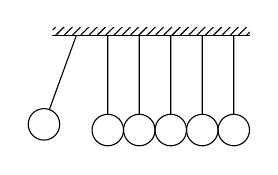
\begin{tikzpicture}[line cap = round, line join = round]
  \def\myang{-110} % between -90 and -180
  
  \draw (-1.5cm, 0) -- (1cm, 0);
  
  \fill[pattern = north east lines] (-1.5cm, 0) rectangle (1cm, 0.1cm);

  \pend{}
  \pend{xshift = 0.4cm}
  \pend{xshift = 0.8cm}
  \pend{xshift = -0.4cm}
  \pend{xshift = -0.8cm}

  \draw (-1.2cm, 0) -- +(\myang:1cm) ++(\myang:1.2cm) circle[radius = 0.2cm];
\end{tikzpicture}
\end{document}
%%% Local Variables:
%%% mode: latex
%%% TeX-master: t
%%% End:
